\documentclass[11pt,a4paper]{article}
\usepackage[margin=2.2cm]{geometry}
\usepackage{graphicx,booktabs,url,amsmath}
\usepackage[hidelinks]{hyperref}
\usepackage{placeins}
\usepackage{float}
\graphicspath{{../../../fullsim_analysis/results/bench/2026-10-27/}}
\newcommand{\us}{\textmu s}
\title{Pedestal noise of the Citiroc front end:\\ menu 1 of 27 October 2026}
\author{J.\,J.~Gómez-Cadenas}
\date{28 October 2026}
\begin{document}
\maketitle

\noindent On 27 October 2026 the noise programme of the Citiroc~1A front end (menu~1) was
repeated on three A5202 boards, 1, 2 and 4, connected to their SiPM matrices through the CAEN
adapter boards and running the upgraded FPGA firmware (0xa7070800). This report gives the
pedestal noise of the three boards, its dependence on the shaping time and on the hold delay,
the comparison with the sessions of 22 and 23 October, and the values to be frozen for the noise
model of the simulation.

\section{Data}

The data are nine pedestal runs (Table~\ref{tab:runs}) with the SiPMs biased at 36.5~V, below
breakdown, a periodic trigger every 1~ms and 10\,000 events per board and run. The DAQ reads the
three boards on one chain, as boards 0, 1 and 2; they are boards 1, 2 and 4 of the bench, and are
named so throughout. The low gain is shaped at 87.5~ns in all runs; the preamplifier gains are
55 in both paths and the peak detectors work in peak-stretch mode. The detectors of boards 2 and
4 were at 24.5 and 25.5~$^\circ$C.

\begin{table}[H]
\centering
\small
\begin{tabular}{llll}
\toprule
Runs & Purpose & HG shaping & HoldDelay \\
\midrule
91, 92, 93 & noise against shaping & 25, 50, 87.5 ns & 0 ns \\
94--98 & pedestal against HoldDelay & 25 ns & 96, 200, 296, 400, 496 ns \\
99 & stability (repeats run 91) & 25 ns & 0 ns \\
\bottomrule
\end{tabular}
\caption{Pedestal runs of 27 October, boards 1, 2 and 4.}
\label{tab:runs}
\end{table}

\section{Method}

For each channel the pedestal is the median of its high-gain value over the run and the
deviation of an event is the value minus the pedestal. The 32 channels of a Citiroc are read at
the same trigger, so the mean deviation of the chip in an event is its common mode, and the noise
of each channel splits into a coherent part, the common mode scaled by the slope $b_i$ of the
channel against it, and an incoherent part, the remainder. The total, coherent and incoherent
noise of a chip are the rms of these three quantities over the channels and the events, after
setting aside the events in which the common mode exceeds six robust widths (jumps of the chip)
and the single-channel outliers beyond five robust widths. The definitions are those of the noise
note.

\section{Results}

\subsection{Pedestals and noise of every channel}

\begin{figure}[H]
\centering
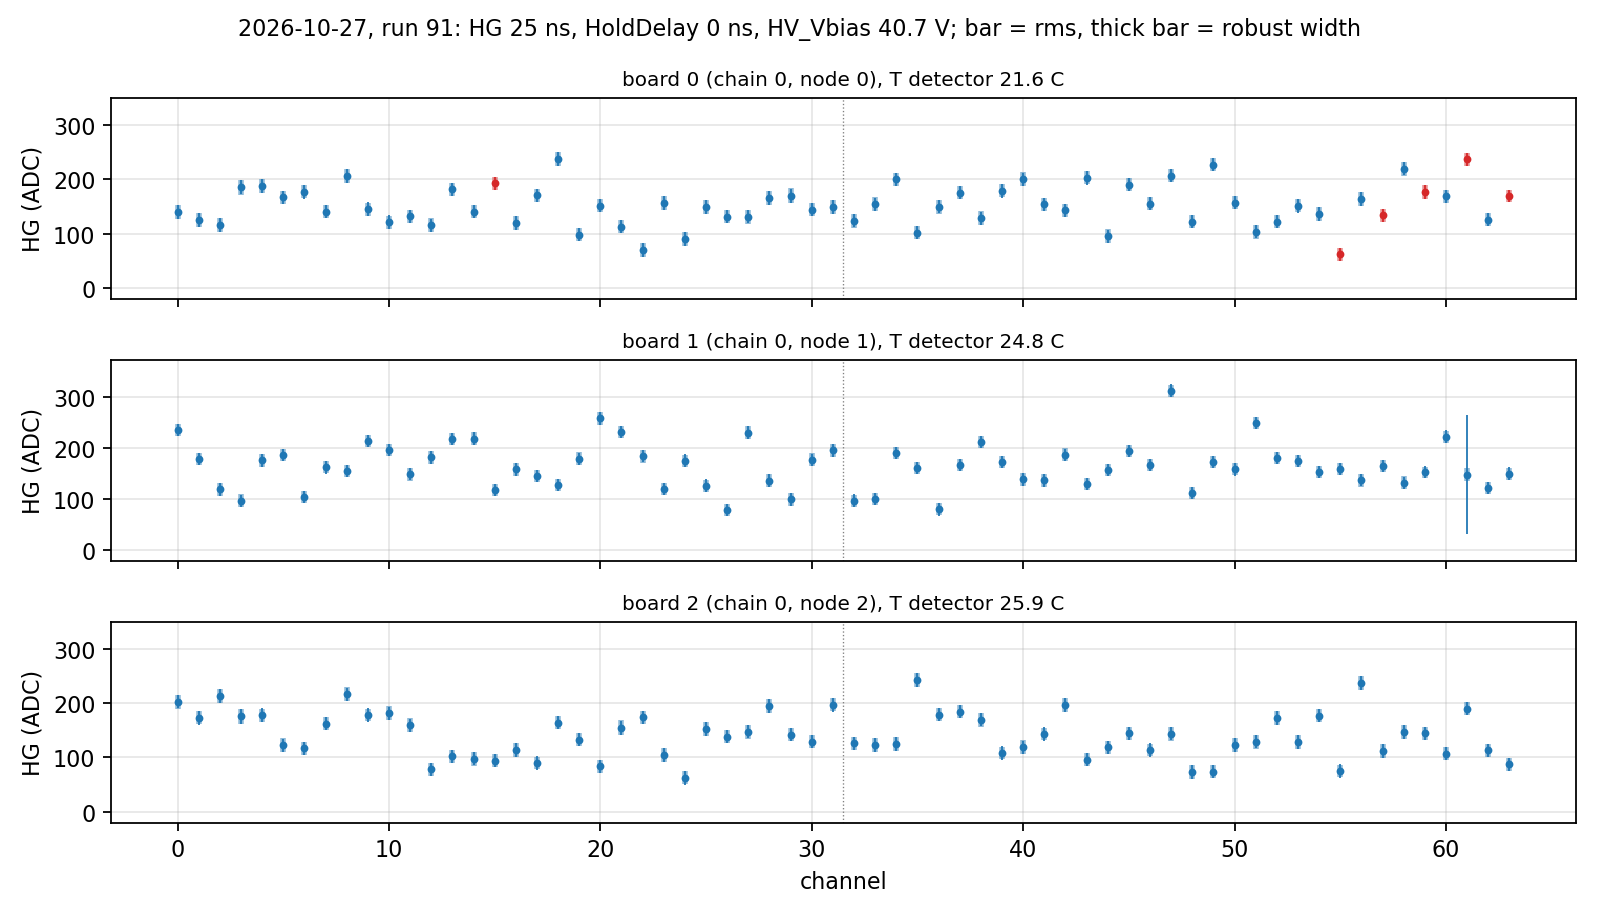
\includegraphics[width=0.92\textwidth]{bench_pedestals.png}
\caption{Run 91 (HG 25~ns, HoldDelay 0): pedestal of the high gain against the channel on boards
1, 2 and 4, with the rms as the error bar.}
\label{fig:pedestals}
\end{figure}

\begin{figure}[H]
\centering
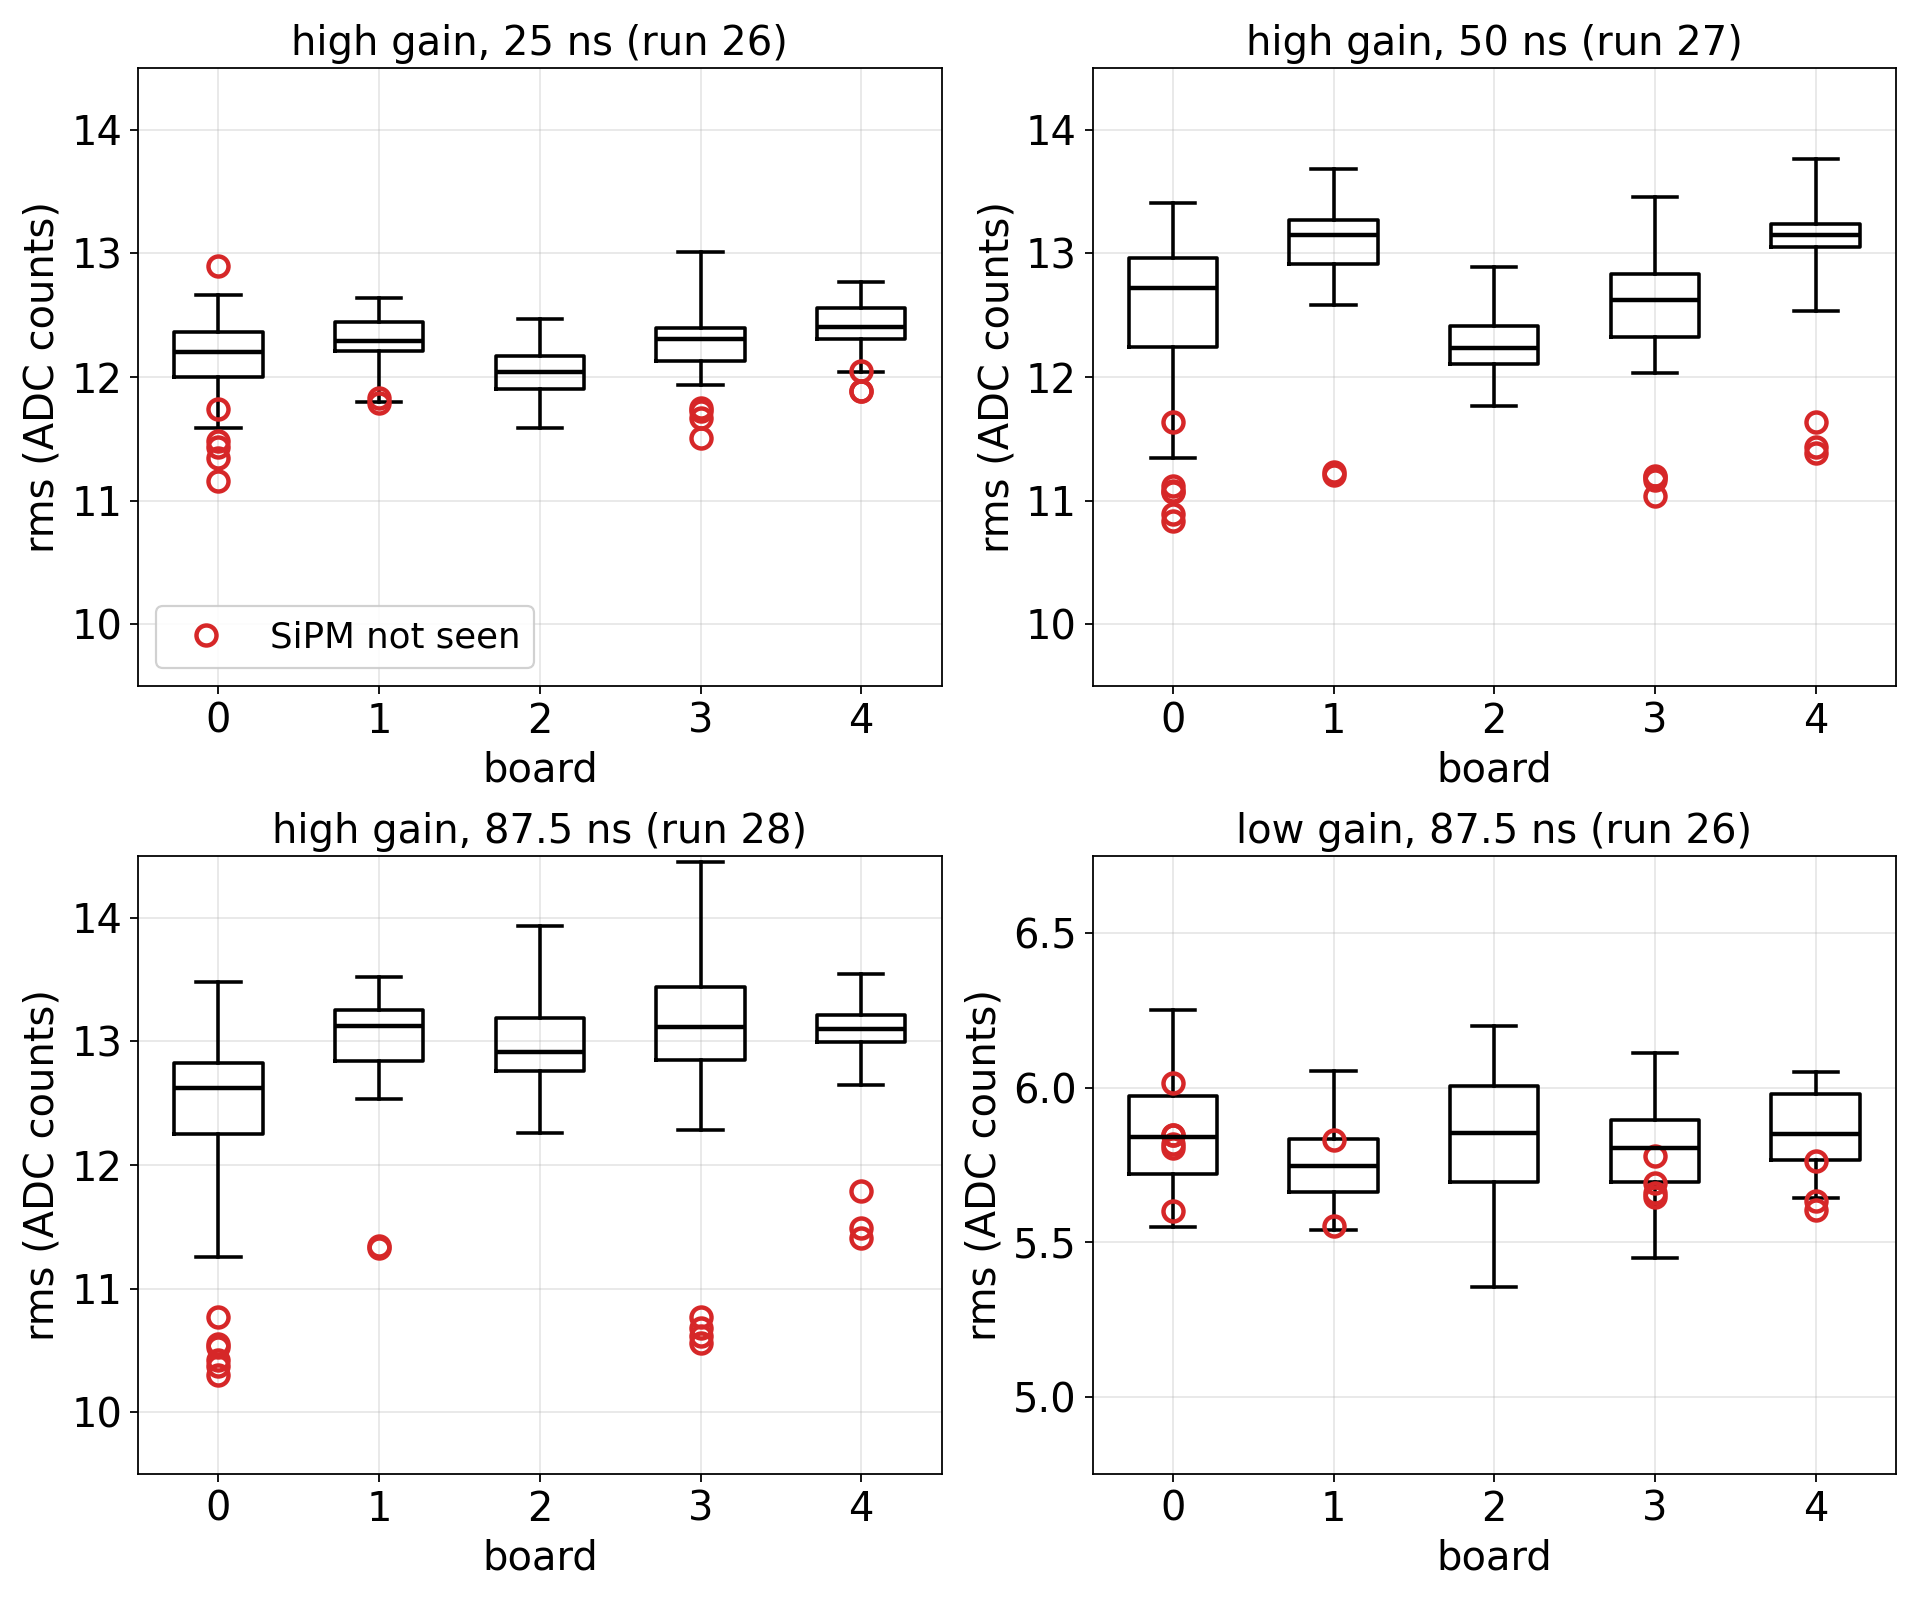
\includegraphics[width=0.85\textwidth]{bench_rms.png}
\caption{Rms of every channel, without jumps and outliers: high gain at 25, 50 and 87.5~ns and
low gain at 87.5~ns, one box per board (quartiles, whiskers to the extremes). The red circles are
the channels that do not see their SiPM.}
\label{fig:rms}
\end{figure}

The pedestals lie between 100 and 300 counts and every channel of the three boards is read
(Figure~\ref{fig:pedestals}). At 25~ns the rms of the high gain is 12.0 to 12.4 counts in the
median of each board, with a spread of about 1~count across the 64 channels, and 5.9~counts in
the low gain (Figure~\ref{fig:rms}). The channels that do not see their SiPM, identified below,
are the quietest of their board at long shaping.

\subsection{Coherent and incoherent noise}

\begin{table}[H]
\centering
\small
\begin{tabular}{llcccccc}
\toprule
day & adapter & board & channels & $\sigma_\mathrm{tot}$ & $\sigma_\mathrm{coh}$ & $\sigma_\mathrm{inc}$ & $\sigma_\mathrm{coh}^2/\sigma_\mathrm{tot}^2$ \\
\midrule
22 Oct & green & 0 & 0--31 & 12.0 & 6.0 & 10.4 & 0.25 \\
22 Oct & green & 0 & 32--63 & 12.3 & 7.0 & 10.2 & 0.32 \\
22 Oct & green & 1 & 32--63 & 12.3 & 6.4 & 10.5 & 0.27 \\
22 Oct & green & 2 & 0--31 & 12.1 & 5.9 & 10.6 & 0.24 \\
22 Oct & green & 2 & 32--63 & 11.9 & 5.9 & 10.3 & 0.25 \\
22 Oct & green & 3 & 0--31 & 12.3 & 6.4 & 10.5 & 0.27 \\
22 Oct & green & 3 & 32--63 & 12.3 & 6.3 & 10.5 & 0.26 \\
22 Oct & green & 4 & 32--63 & 12.4 & 6.3 & 10.7 & 0.26 \\
\midrule
23 Oct & red & 0 & 0--31 & 12.1 & 6.0 & 10.4 & 0.25 \\
23 Oct & red & 0 & 32--63 & 12.5 & 7.2 & 10.2 & 0.33 \\
23 Oct & red & 1 & 0--31 & 10.7 & 5.5 & 9.1 & 0.26 \\
23 Oct & red & 1 & 32--63 & 12.3 & 6.5 & 10.5 & 0.28 \\
\midrule
27 Oct & red & 1 & 0--31 & 12.7 & 6.7 & 10.7 & 0.28 \\
27 Oct & red & 1 & 32--63 & 12.1 & 6.3 & 10.4 & 0.27 \\
27 Oct & red & 2 & 0--31 & 12.1 & 5.9 & 10.6 & 0.24 \\
27 Oct & red & 2 & 32--63 & 11.9 & 6.0 & 10.3 & 0.25 \\
27 Oct & red & 4 & 0--31 & 12.4 & 6.2 & 10.8 & 0.25 \\
27 Oct & red & 4 & 32--63 & 12.4 & 6.4 & 10.6 & 0.27 \\
\bottomrule
\end{tabular}

\caption{Total, coherent and incoherent noise of the high gain and the coherent fraction of the
variance, per chip, at 25~ns and HoldDelay 0, in ADC counts: the three sessions.}
\label{tab:chips}
\end{table}

The six chips of 27 October lie within 11.9 to 12.7~counts in total noise, 5.9 to 6.7 coherent
and 10.3 to 10.8 incoherent (Table~\ref{tab:chips}). The coherent part carries 24 to 28\% of the
variance. The two chips of a board share their common mode with a correlation of 0.59 to 0.64;
the common modes of different boards are uncorrelated (correlation between $-0.01$ and 0.02).
No chip shows a jump in any of the nine runs.

\subsection{Dependence on the shaping time}

\begin{figure}[H]
\centering
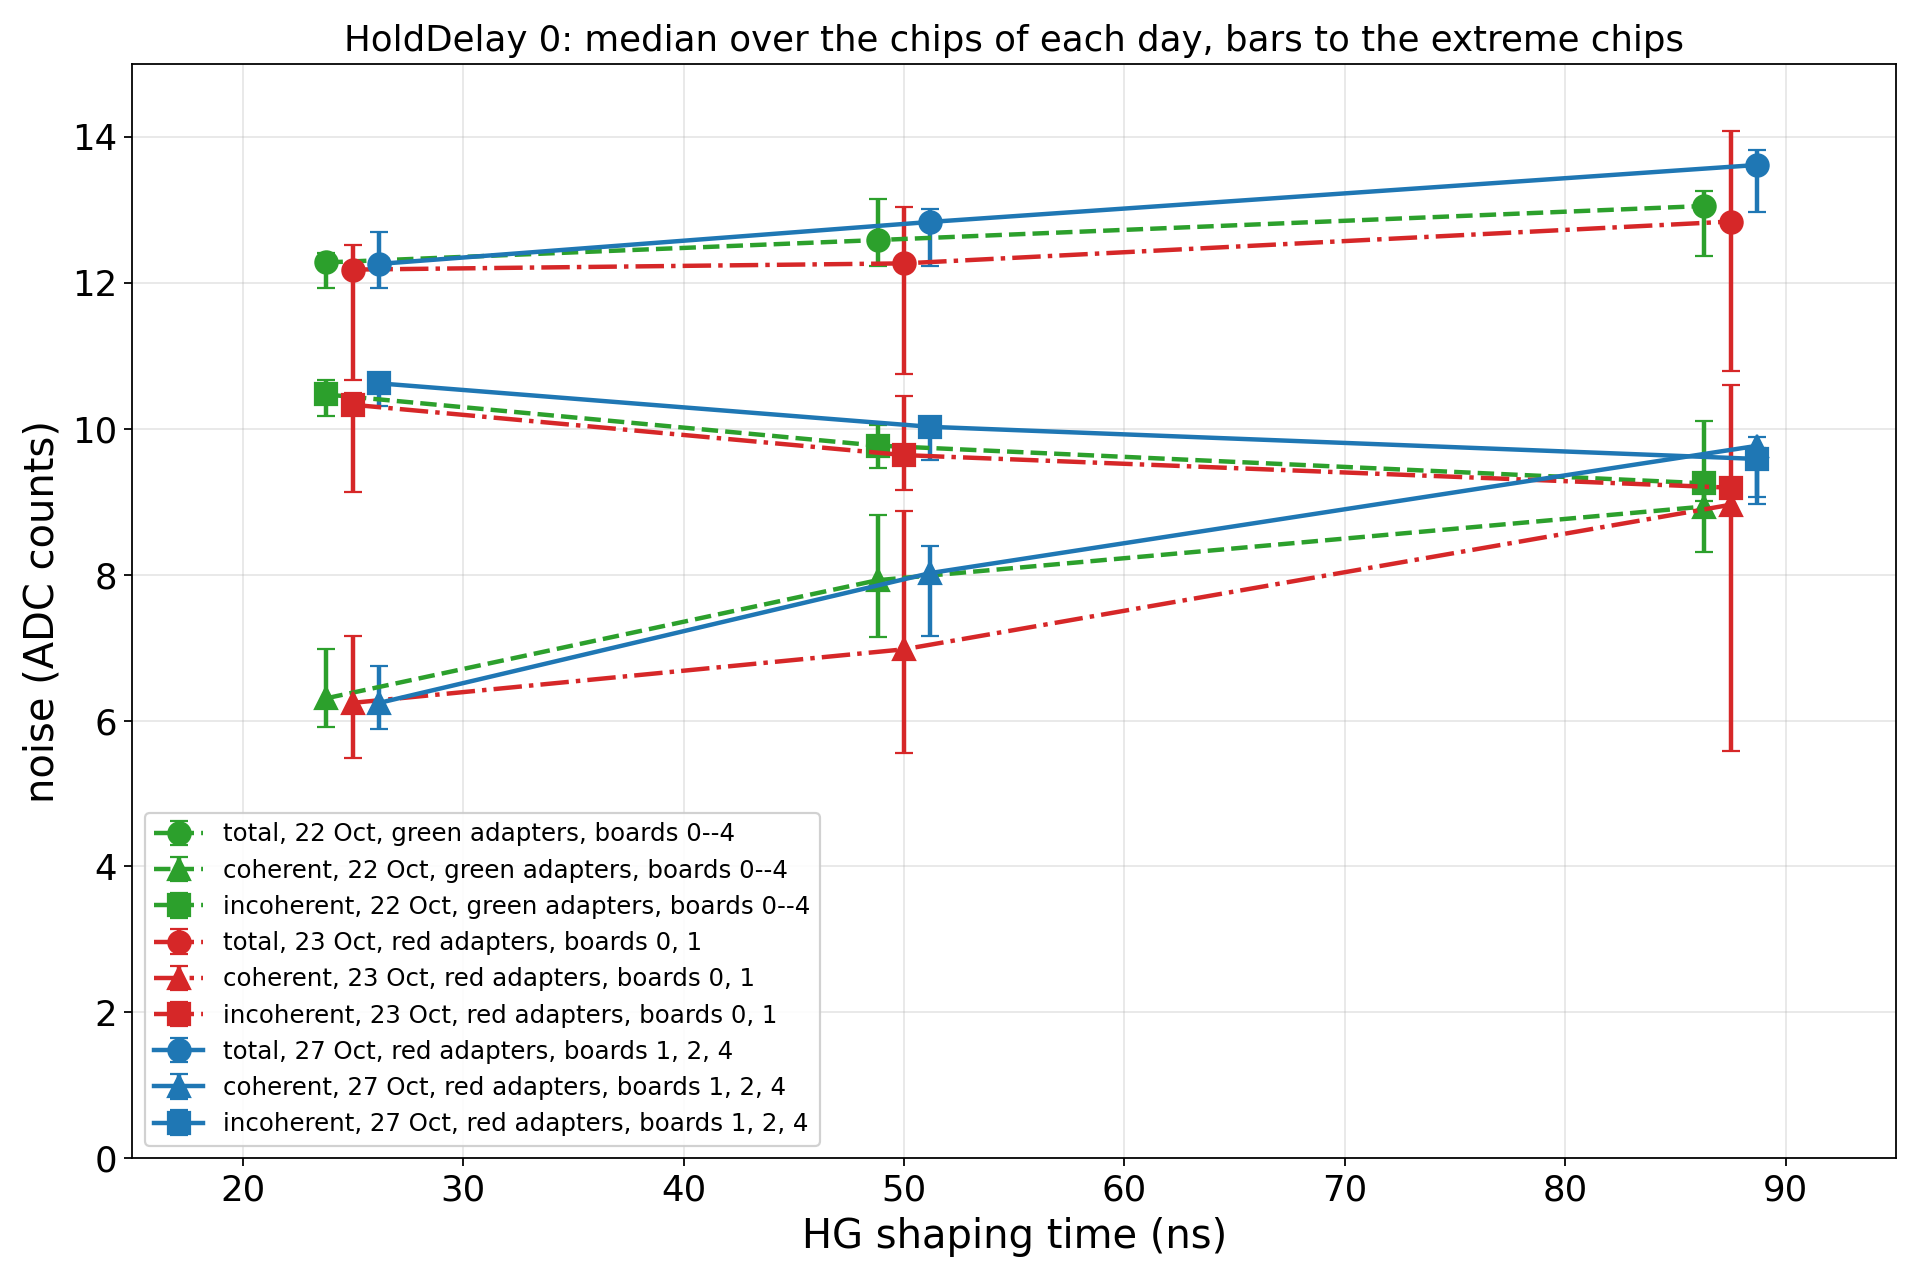
\includegraphics[width=0.8\textwidth]{compare_days_shaping.png}
\caption{Total, coherent and incoherent noise of the high gain against the shaping time at
HoldDelay 0: median over the chips of each session, bars to the extreme chips.}
\label{fig:shaping}
\end{figure}

\begin{table}[H]
\centering
\small
\begin{tabular}{llcccc}
\toprule
day & shaping & chips & $\sigma_\mathrm{tot}$ & $\sigma_\mathrm{coh}$ & $\sigma_\mathrm{inc}$ \\
\midrule
22 Oct & 25 ns & 8 & 12.3 (11.9--12.4) & 6.3 (5.9--7.0) & 10.5 (10.2--10.7) \\
22 Oct & 50 ns & 8 & 12.6 (12.2--13.2) & 7.9 (7.2--8.8) & 9.8 (9.5--10.0) \\
22 Oct & 87.5 ns & 8 & 13.1 (12.4--13.3) & 8.9 (8.3--9.4) & 9.3 (9.0--10.1) \\
\midrule
23 Oct & 25 ns & 4 & 12.2 (10.7--12.5) & 6.2 (5.5--7.2) & 10.3 (9.1--10.5) \\
23 Oct & 50 ns & 4 & 12.3 (10.7--13.0) & 7.0 (5.6--8.9) & 9.6 (9.2--10.4) \\
23 Oct & 87.5 ns & 4 & 12.8 (10.8--14.1) & 9.0 (5.6--10.6) & 9.2 (9.1--9.3) \\
\midrule
27 Oct & 25 ns & 6 & 12.3 (11.9--12.7) & 6.2 (5.9--6.7) & 10.6 (10.3--10.8) \\
27 Oct & 50 ns & 6 & 12.8 (12.2--13.0) & 8.0 (7.2--8.4) & 10.0 (9.6--10.1) \\
27 Oct & 87.5 ns & 6 & 13.6 (13.0--13.8) & 9.8 (9.0--9.9) & 9.6 (9.1--9.7) \\
\bottomrule
\end{tabular}

\caption{Median over the chips and range of the three components at HoldDelay 0, ADC counts,
for each session and shaping.}
\label{tab:summary}
\end{table}

The total noise grows from 12.3 to 12.8 and 13.6~counts between 25, 50 and 87.5~ns
(Figure~\ref{fig:shaping}, Table~\ref{tab:summary}). The growth is in the coherent part, 6.2,
8.0 and 9.8~counts, while the incoherent part falls from 10.6 to 10.0 and 9.6. The low gain,
shaped at 87.5~ns in all runs, has 0.48, 0.46 and 0.43 of the total noise of the high gain at
25, 50 and 87.5~ns.

\subsection{Dependence on the hold delay}

\begin{figure}[H]
\centering
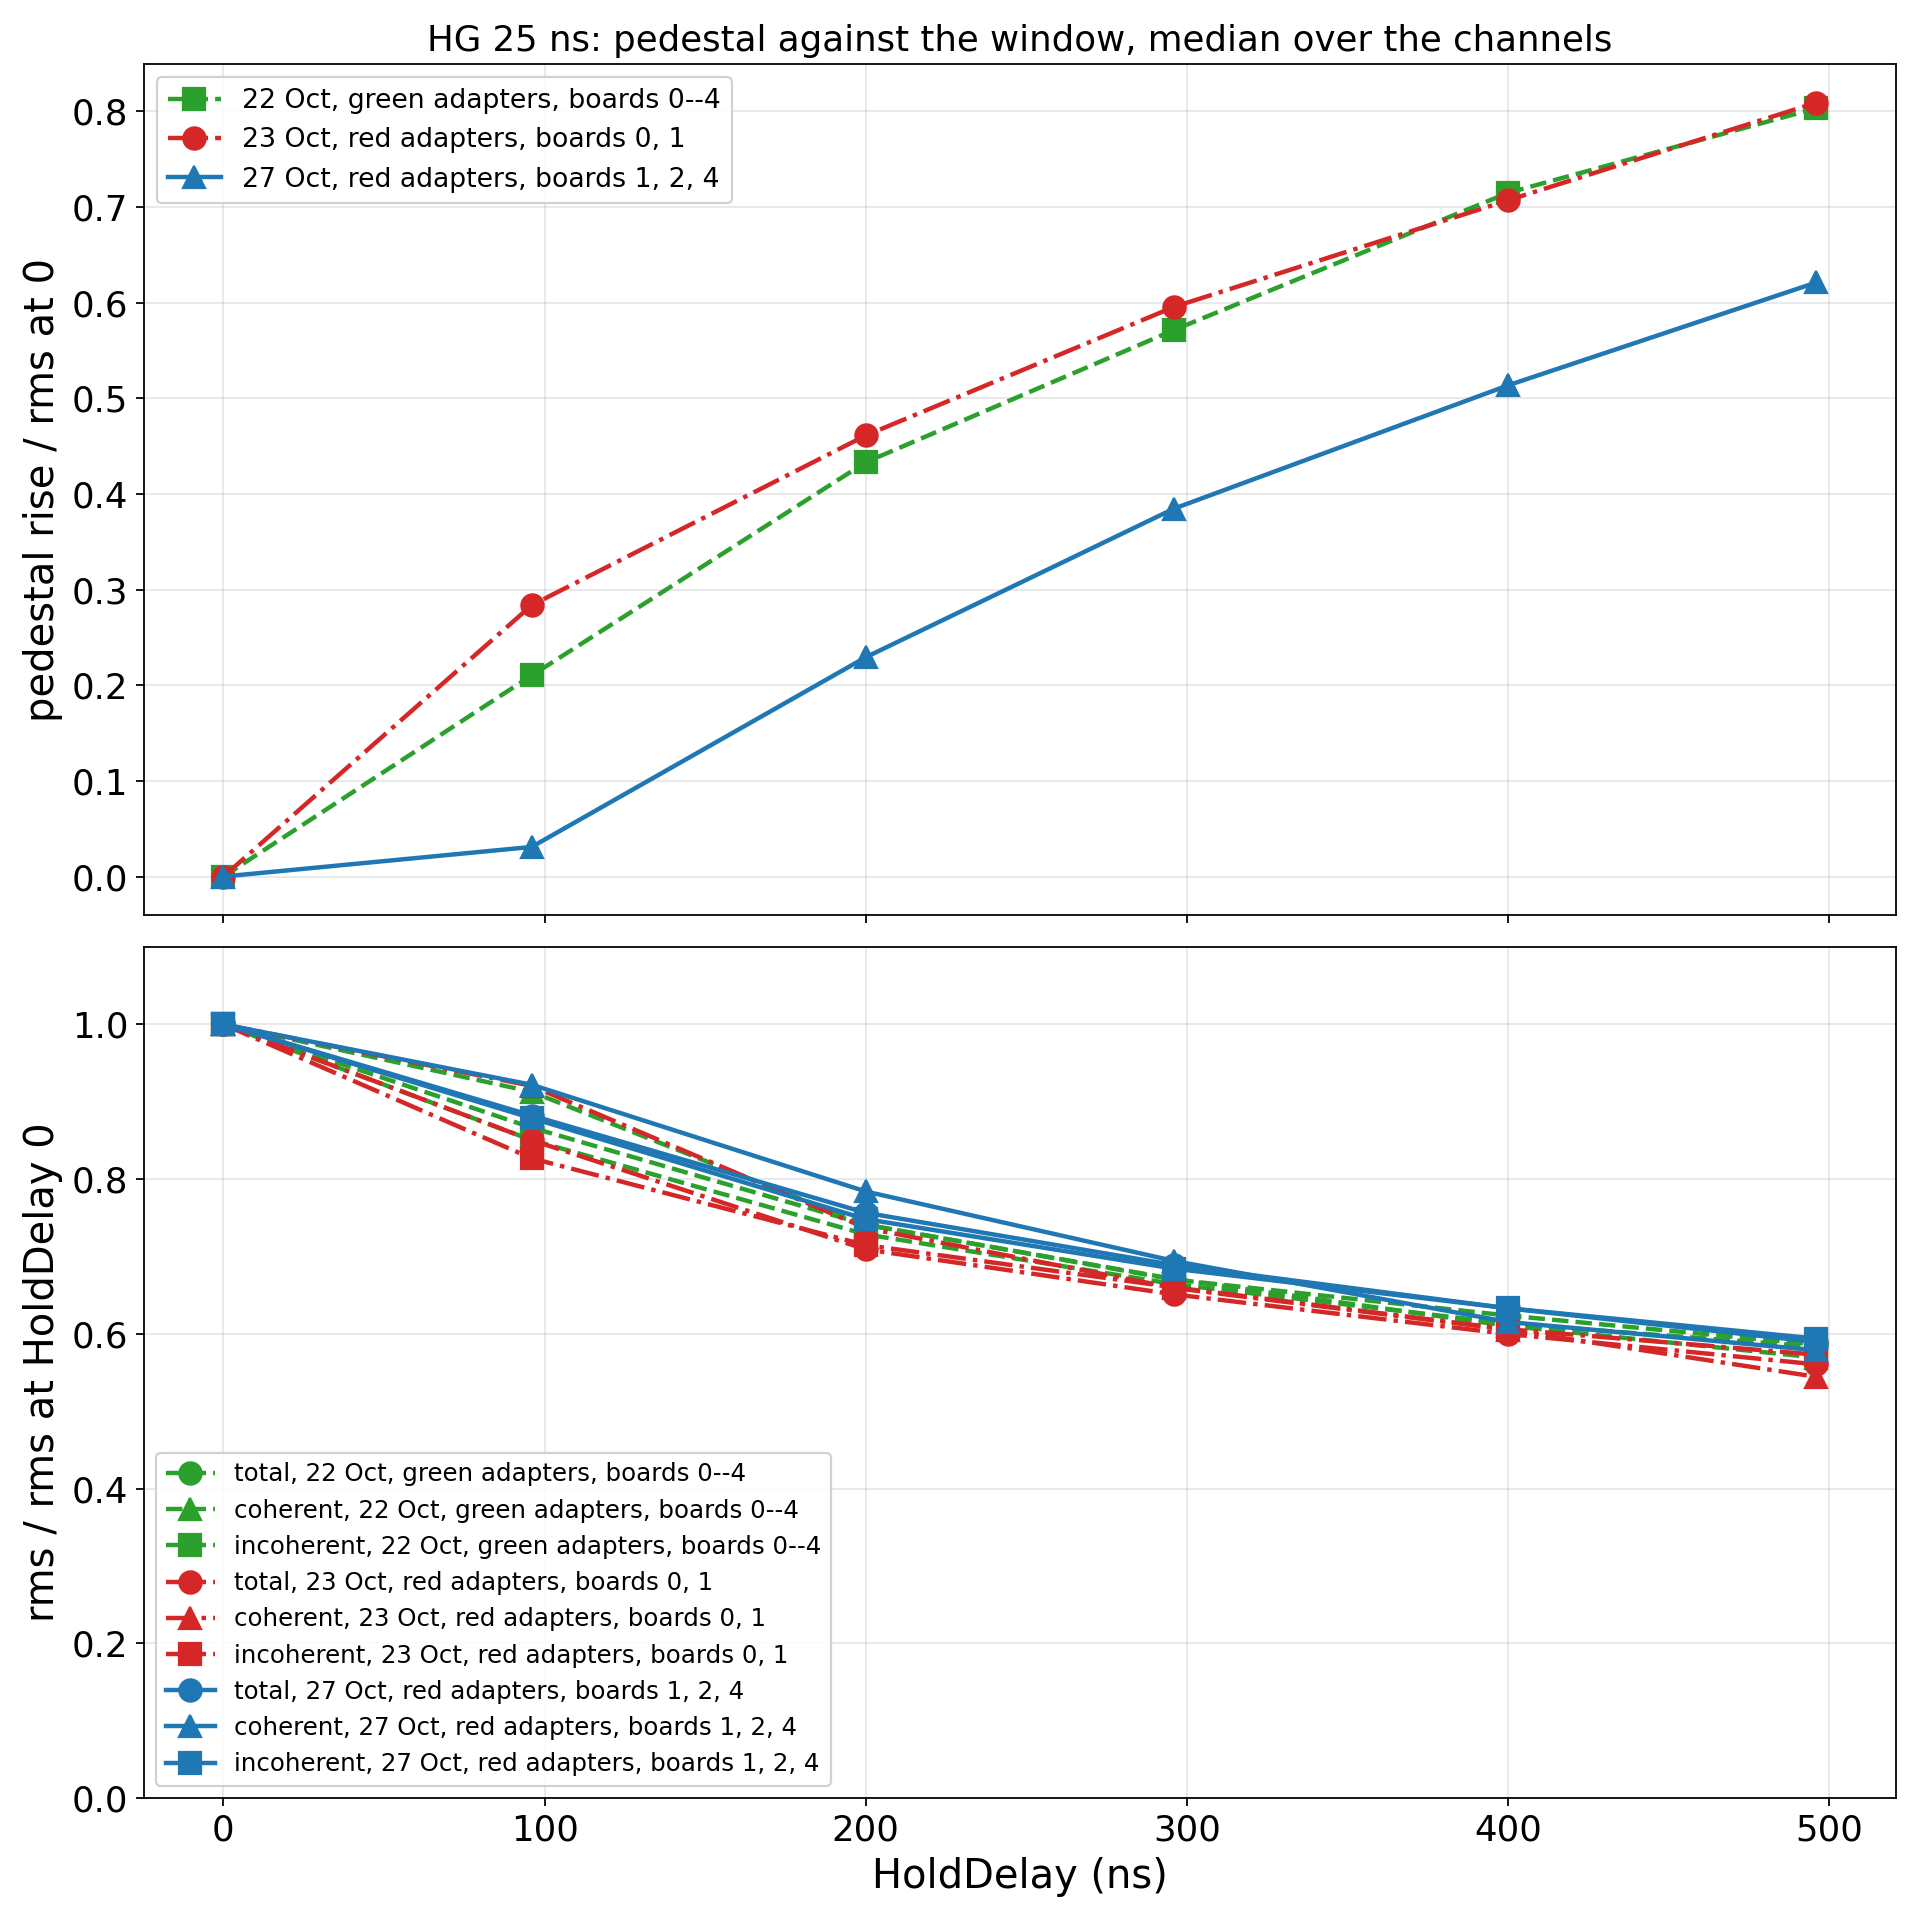
\includegraphics[width=0.72\textwidth]{compare_days_holddelay.png}
\caption{High gain at 25~ns against HoldDelay. Top: rise of the pedestal from its value at
HoldDelay 0, in units of the rms at HoldDelay 0, median over the channels. Bottom: total, coherent
and incoherent rms relative to HoldDelay 0, median over the chips.}
\label{fig:hold}
\end{figure}

With the peak detector in peak-stretch mode the stored value is the maximum of the shaped signal
over the window opened by the hold delay. At 25~ns the rms of the noise falls to 0.88, 0.76,
0.69, 0.63 and 0.59 of its value at HoldDelay 0 for delays of 96, 200, 296, 400 and 496~ns, and
the coherent and incoherent parts fall together (Figure~\ref{fig:hold}, bottom). The pedestal
rises with the window by 0.4, 2.9, 4.7, 6.3 and 7.7~counts, that is 0.62 of the rms at 496~ns,
with no rise up to 96~ns (Figure~\ref{fig:hold}, top).

\subsection{Channels that do not see their SiPM}

\begin{figure}[H]
\centering
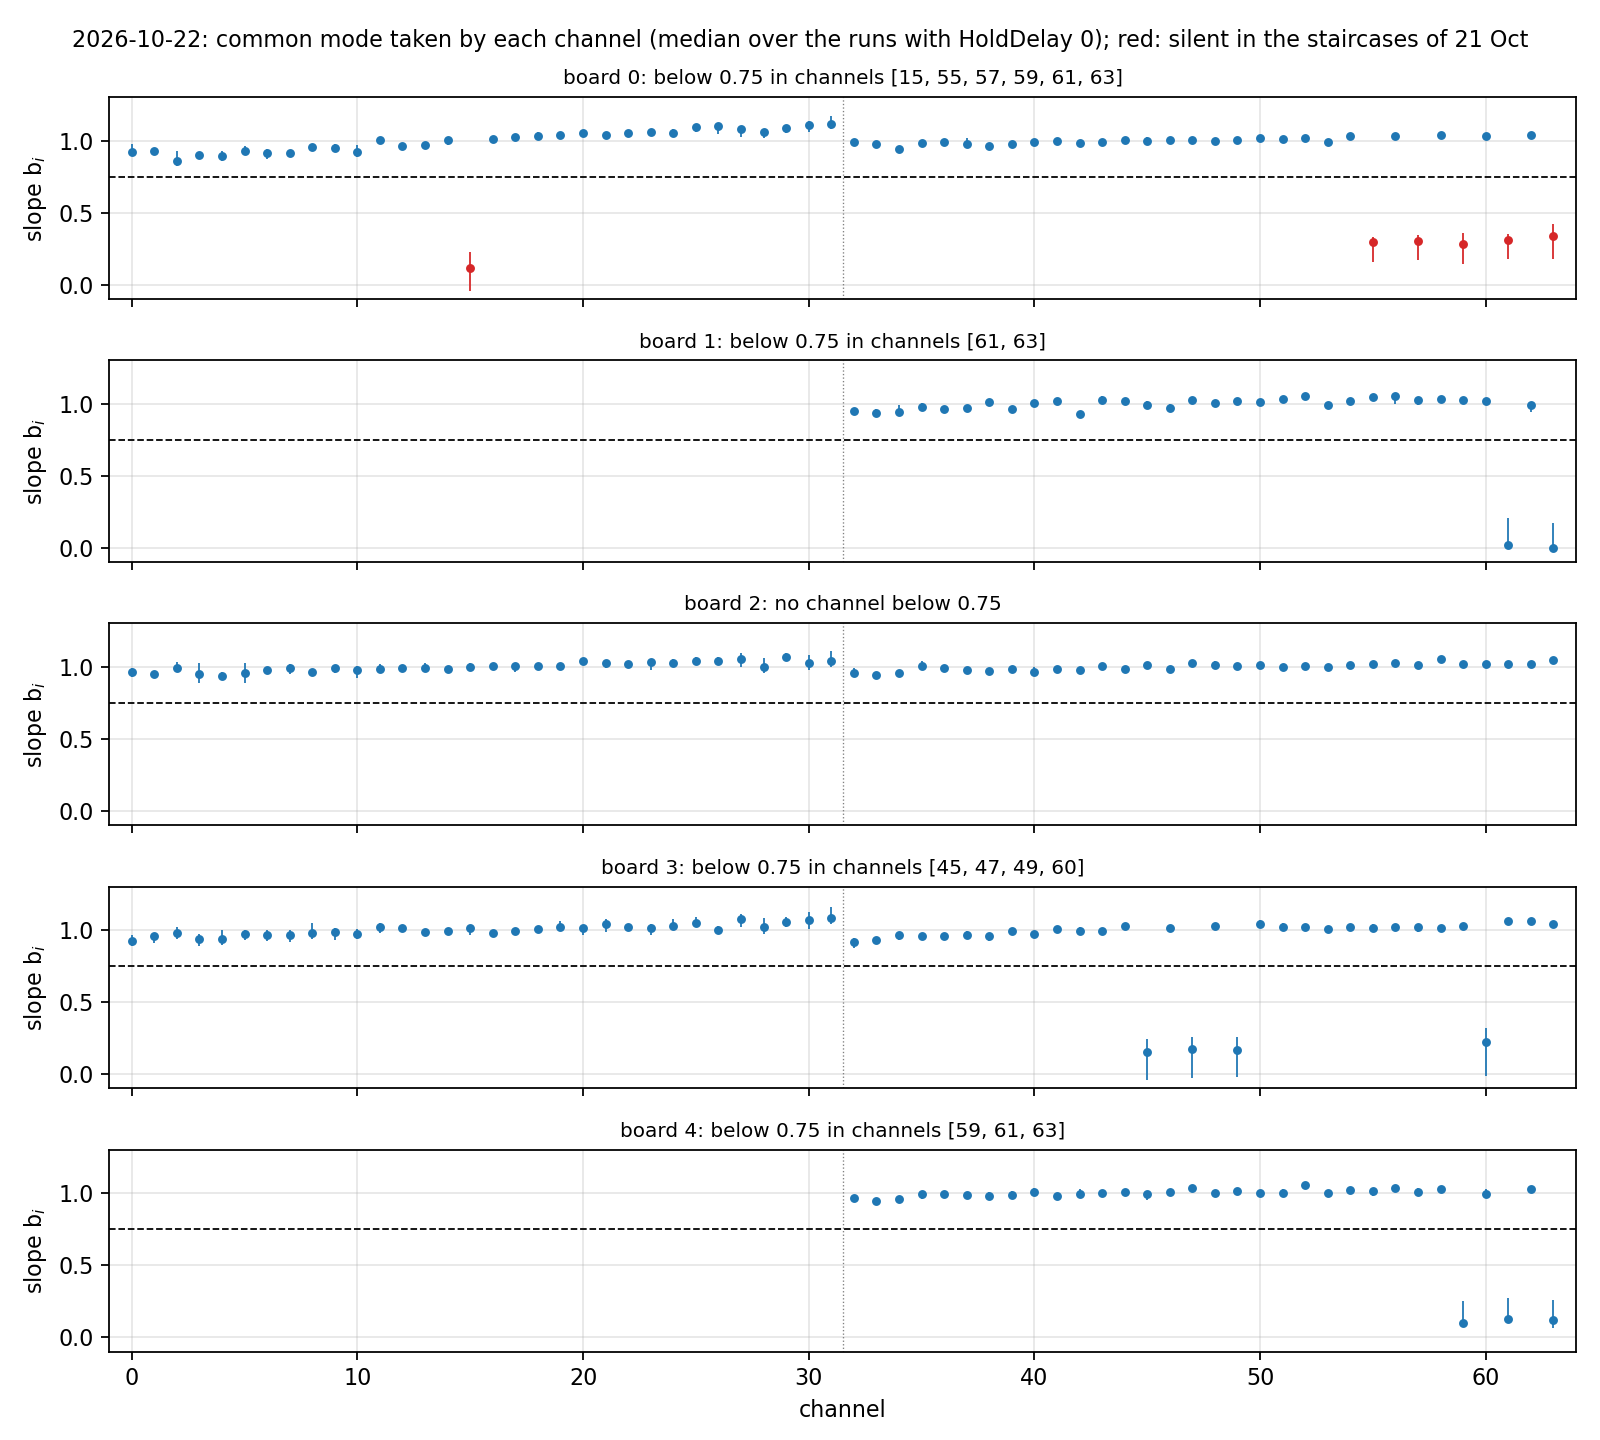
\includegraphics[width=0.9\textwidth]{bench_slopes.png}
\caption{Slope $b_i$ of each channel against the common mode of its chip, median over the runs
with HoldDelay 0 (bars to the extremes), boards 1, 2 and 4. The dashed line is the cut at 0.75.}
\label{fig:slopes}
\end{figure}

The common mode enters the chip through the SiPMs, so a channel whose SiPM is not connected
takes a slope well below one (Figure~\ref{fig:slopes}). On board 1 channels 61 and 63 have slopes
below 0.2, on board 4 channels 3, 59, 61 and 63, and every other channel of the three boards is
above 0.85. Board 2 has no such channel. Channel 62 of board 1, blind on 23 October, takes the
full common mode on 27 October.

\section{Comparison with 22 and 23 October}

The sessions of 22 October (boards 0 to 4, adapter boards made in-house, earlier firmware) and
23 October (boards 0 and 1, CAEN adapter boards) measured the same noise, chip by chip, as the
session of 27 October (Table~\ref{tab:chips}): over the eighteen chips of the three sessions the
total noise at 25~ns spans 10.7 to 12.7~counts, with sixteen chips between 11.9 and 12.7, and the
coherent fraction 0.24 to 0.33. The dependences on the shaping (Figure~\ref{fig:shaping}) and the
narrowing of the rms with the hold delay (Figure~\ref{fig:hold}, bottom) coincide within the
spread of the chips. The noise of the Citiroc front end is therefore a property of the board and
the chip, the same on the five boards, with either adapter board and either firmware.

One quantity differs: the rise of the pedestal with the hold delay is slower on 27 October,
0.62 of the rms at 496~ns against 0.80 on 22 and 23 October, and absent up to 96~ns where the
earlier sessions had 0.21 to 0.28 (Figure~\ref{fig:hold}, top).

\section{Values for the noise model}

The following are measured on the five boards and frozen for the noise model of the simulation,
in ADC counts of the high gain with the preamplifier gain at 55:
\begin{enumerate}
\item At 25~ns and HoldDelay 0, per channel: total noise 12.3, coherent 6.2, incoherent 10.6.
\item Against the shaping time, at HoldDelay 0: total 12.3, 12.8, 13.6 and coherent 6.2, 8.0,
  9.8 at 25, 50 and 87.5~ns; the incoherent part 10.6, 10.0, 9.6.
\item Against the hold delay, at 25~ns: the rms of both components scaled by 1.00, 0.88, 0.76,
  0.69, 0.63 and 0.59 at 0, 96, 200, 296, 400 and 496~ns.
\item The coherent component is common to the 64 channels of a board, with a correlation of
  0.6 between its two chips and none between boards.
\item The low gain at 87.5~ns has 0.46 of the noise of the high gain.
\item Boards 1 and 4 have, respectively, two and four channels without signal from their SiPM.
\end{enumerate}
The conversion of these values to photoelectrons takes the single-photoelectron gain from the
calibration of menu~3.

\end{document}
